\documentclass[../DD.tex]{subfiles}
\graphicspath{{\subfix{../assets}}}

\usepackage{geometry}

\begin{document}
    \subsection{Implementation Plan}
        In order to increase the pace of our development, prioritizing the parallelization of various components becomes a top priority. A recommended strategy involves adopting a bottom-up approach, therefore focusing on foundational components with higher dependencies and subjecting them to rigorous testing. This testing will be initially performed by unit testing, since incorporating this kind of testing during the development phase will ensure the construction of a robust application infrastructure, thereby mitigating the need for extensive revisions of previous work. Additionally, early detection of bugs and errors is facilitated through unit testing, preventing instances where errors may necessitate a comprehensive overhaul of the entire implementation.

    \subsection{Integration strategy}
        Considering the architecture of our system and the implementation plan in place, the most rational integration and testing strategy would be bottom-up. This approach, on the whole, facilitates thorough testing at each level, the early identification of issues before they become too widespread. Moreover, bottom-up encourages modularity and reusability. Finally, thanks to its inherent characteristics, bottom-up also facilitates the seamless addition of features to the subsystem as needed.\\
        Components not yet implemented are simulated via test drivers that will be later replaced by the actual component.\\
        In the following section the order of development, integration and testing of the  components is defined. Components not yet implemented will be simulated with test drivers or stubs that will be later replaced by the actual component once it's actually developed.
        \newpage

        \newgeometry{top = 3em}
        \begin{figure}[h!]
            \centering
            \hspace*{-1cm}
            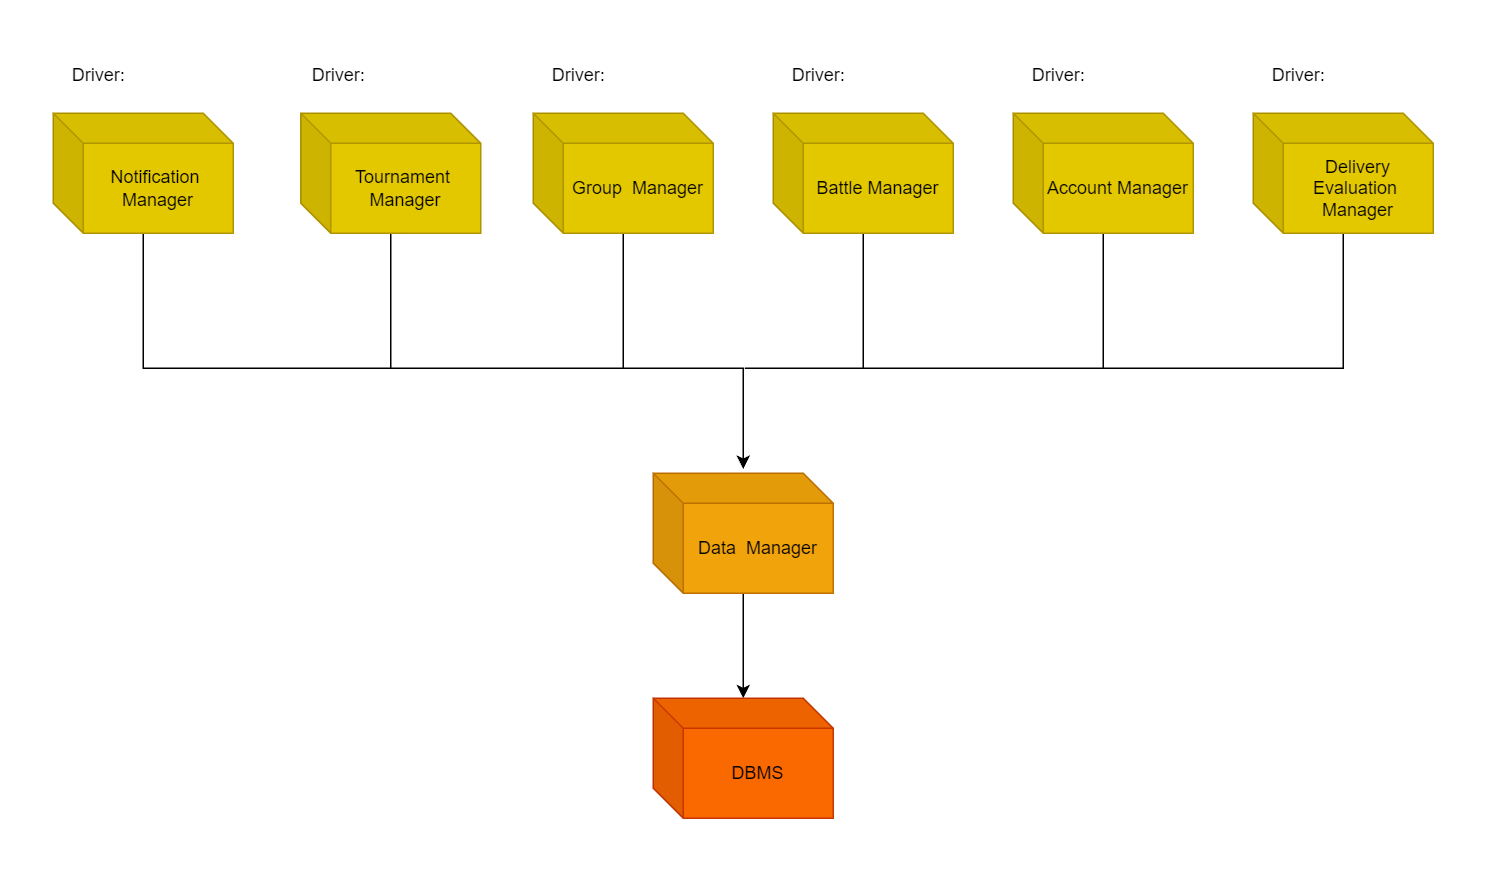
\includegraphics[width=1.05\textwidth]{../assets/section_5/1.png}
            \caption{Integration of Data Manager}
        \end{figure}

        \begin{figure}[H]
            \centering
            \hspace*{-1cm}
            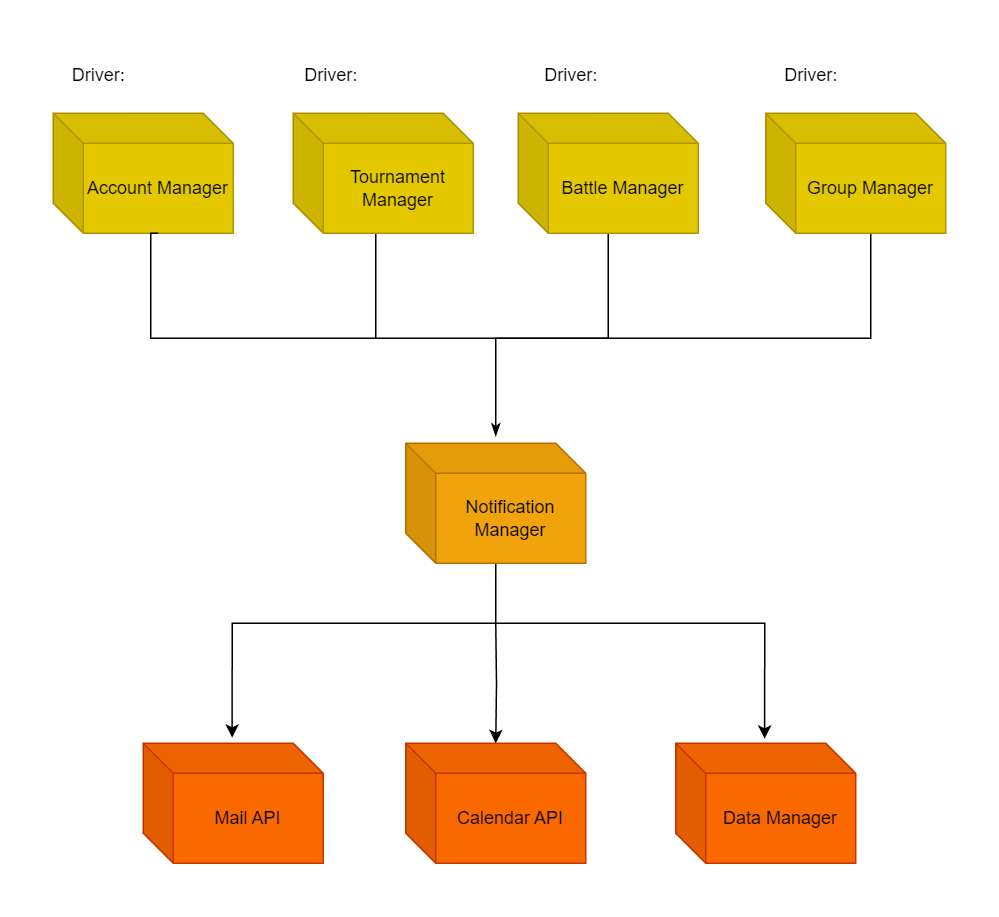
\includegraphics[width=0.8\textwidth]{../assets/section_5/2.png}
            \caption{Integration of Notification Manager}
        \end{figure}
        \newpage

        \begin{figure}[h!]
            \centering
            \hspace*{-1cm}
            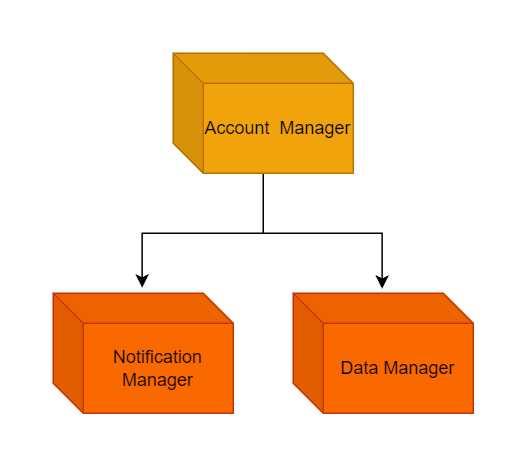
\includegraphics[width=0.55\textwidth]{../assets/section_5/3.png}
            \caption{Integration of Account Manager}
        \end{figure}

        \begin{figure}[h!]
            \centering
            \hspace*{-1cm}
            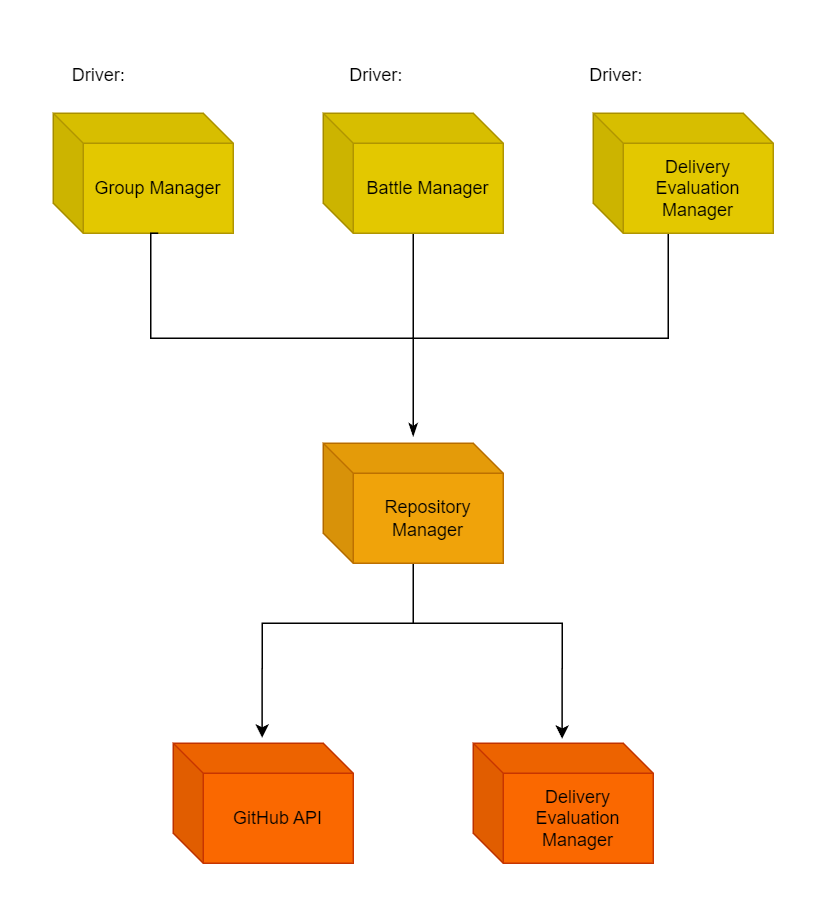
\includegraphics[width=0.65\textwidth]{../assets/section_5/4.png}
            \caption{Integration of Repository Manager}
        \end{figure}
        \newpage

        \begin{figure}[h!]
            \centering
            \hspace*{-1cm}
            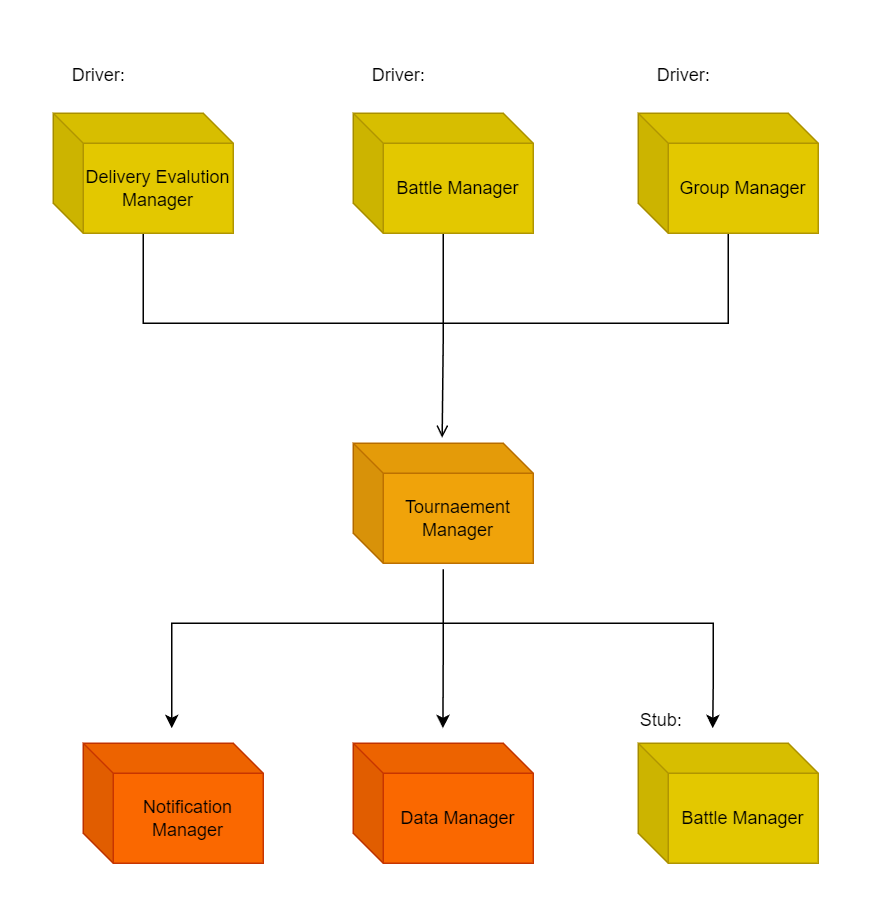
\includegraphics[width=0.65\textwidth]{../assets/section_5/5.png}
            \caption{Integration of Tournament Manager}
        \end{figure}

        \begin{figure}[h!]
            \centering
            \hspace*{-1cm}
            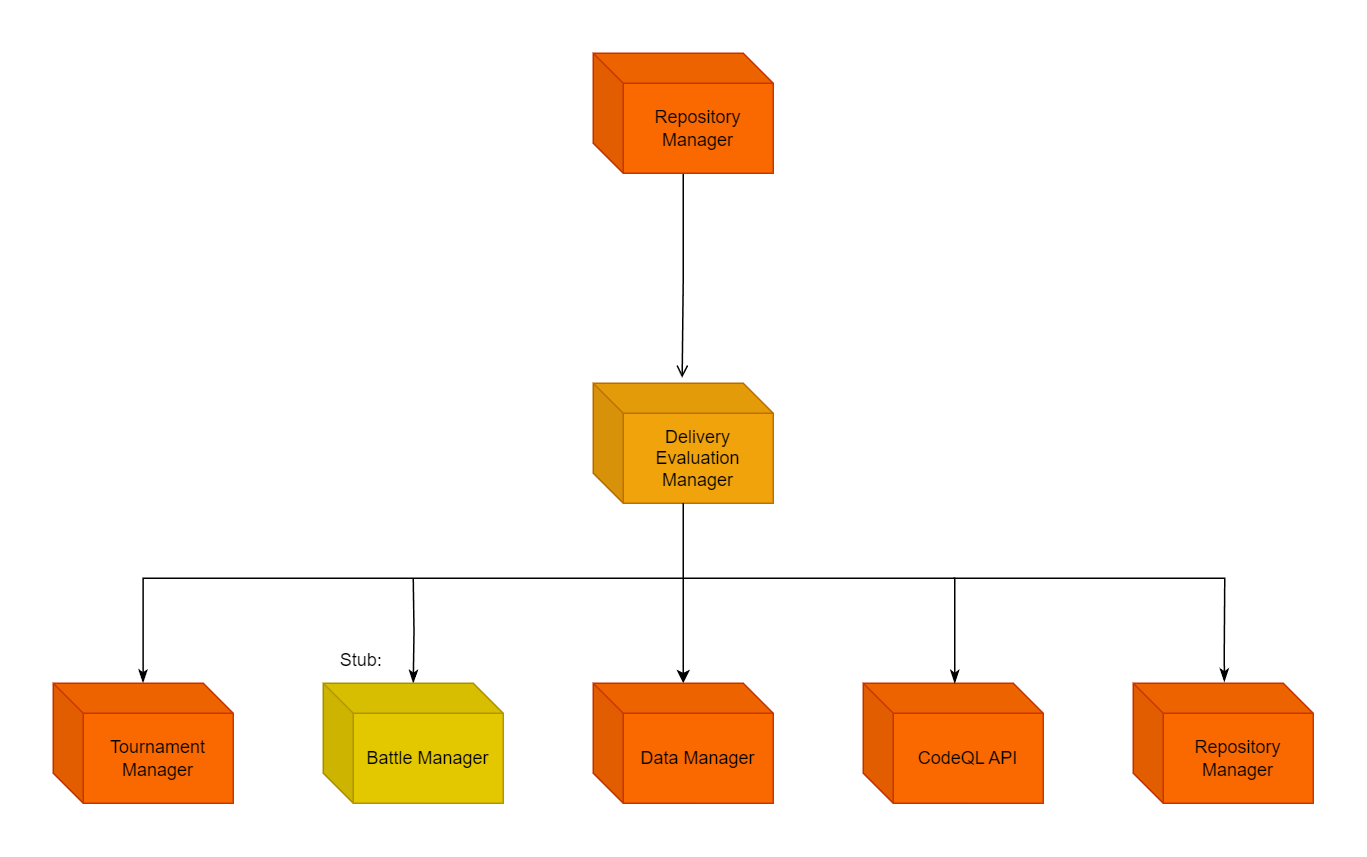
\includegraphics[width=0.9\textwidth]{../assets/section_5/6.png}
            \caption{Integration of Delivery Evaluation Manager}
        \end{figure}
        \newpage

        \begin{figure}[h!]
            \centering
            \hspace*{-1cm}
            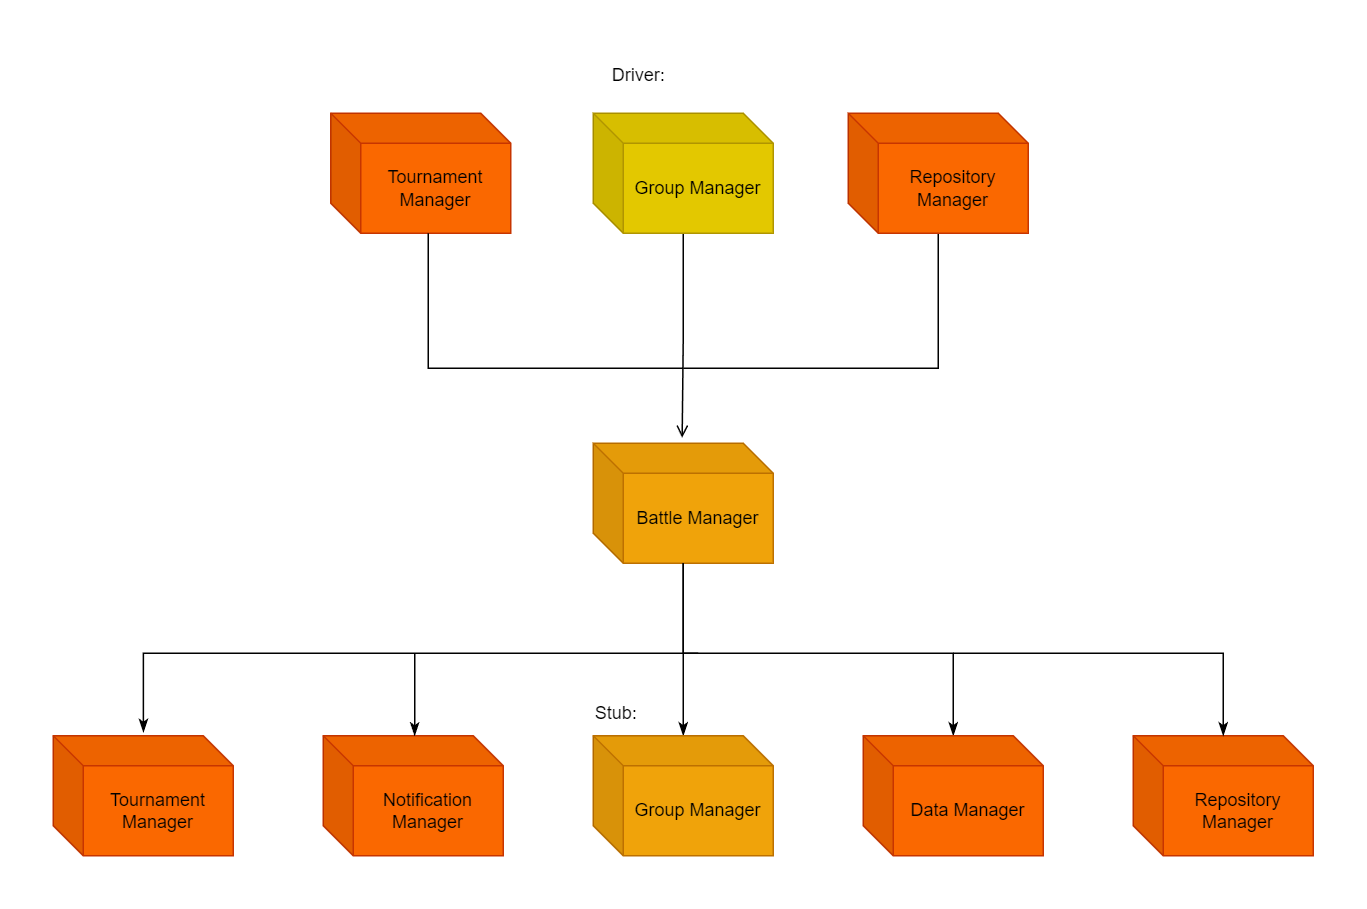
\includegraphics[width=1\textwidth]{../assets/section_5/7.png}
            \caption{Integration of Battle Manager}
        \end{figure}

        \begin{figure}[h!]
            \centering
            \hspace*{-1cm}
            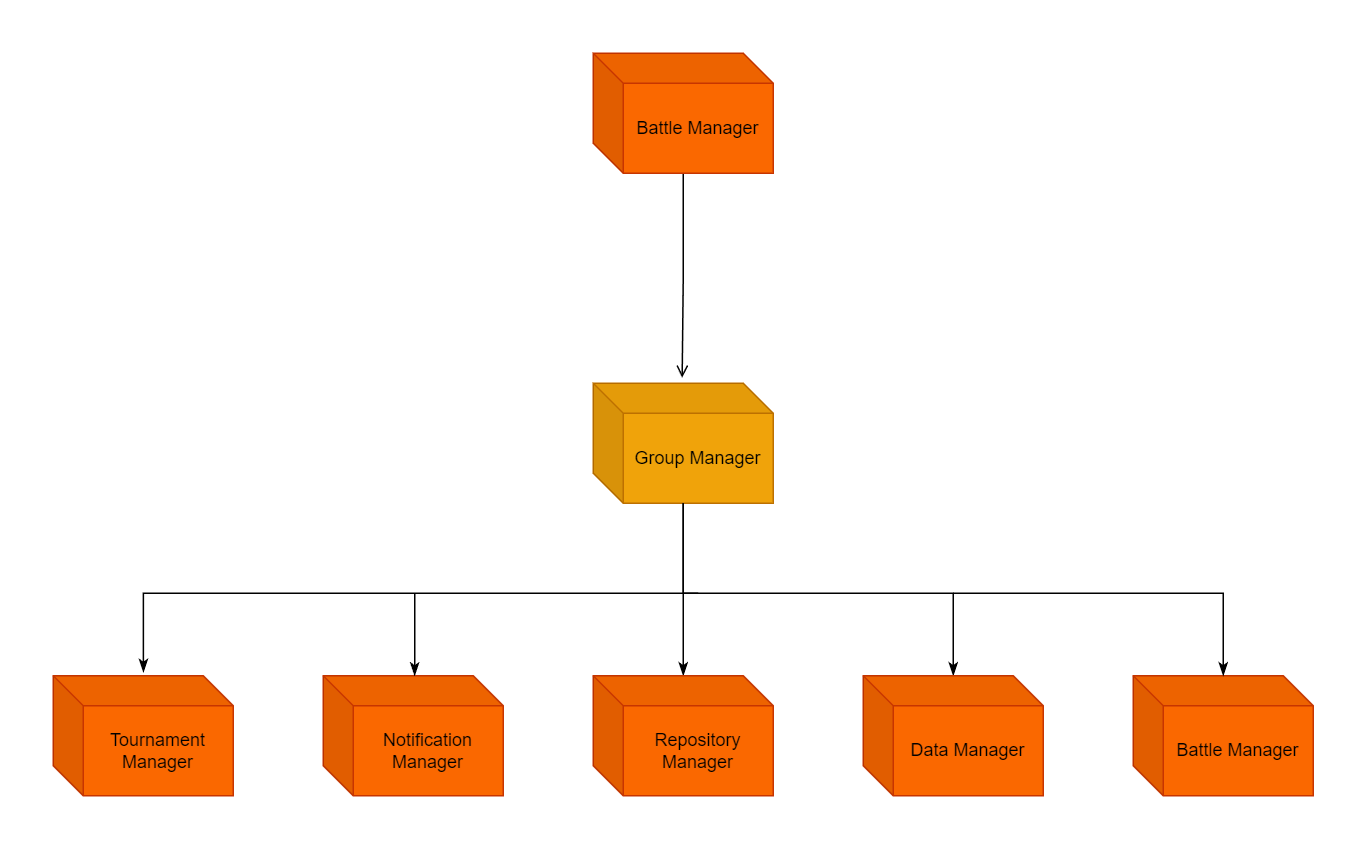
\includegraphics[width=1\textwidth]{../assets/section_5/8.png}
            \caption{Integration of Group Manager}
        \end{figure}
    \restoregeometry
        
    \subsection{System testing}
        Once the individual testing for each component is completed, and it's verified as operational, the last phase involves evaluating the system as a cohesive entity. Therefore, we need to conduct comprehensive testing on the entire system before its deployment and fix any issues that might negatively affect our functionalities or our user experience. For these reasons, we'll run specific tests to assess the complete system's performance, stability, security, and usability.\\
        A crucial aspect of this evaluation will be the performance testing of the system, particularly under high workload conditions, to determine its capability to handle multiple requests concurrently. Furthermore, given the potential for a substantial user base, usability testing will also be of paramount importance, for example, after the application has been developed, we could ask a heterogeneous group of users to complete some surveys about its intuitiveness and user-friendliness. In the event of very negative feedback, a complete UI overhaul may be necessary.

\end{document}